\input preamble.tex
\noindent
\section*{Stasjon 7 - Byggautomasjon}

\vskip 5pt

På denne stasjonen skal du lære om komponenter som normalt brukes i et byggautomatiseringsanlegg. Du må også ta i bruk en ukjent PLS. Dette er noe du som automatikker ofte kan komme borti. Denne PLS-en følger standarden EN-60131-3 for programmering på samme måte som Codesys, slik at du vil etterhver finne likheter i oppbygningen, fordi om du ikke finner funksjonene i de samme menyene. 

Kompetansemål:

planlegge, programmere, montere og idriftsette programmerbare styresystemer

endre og tilpasse skjermbilder for grensesnitt mellom menneske og maskin

anvende ulike elektroniske kommunikasjonssystemer i automatiserte anlegg

montere, konfigurere, kalibrere og idriftsettelse digitale og analoge målesystemer

Dette arbeidsoppdraget består at følgende oppdrag:
\begin{enumerate}
	\item IO-sjekk av alle digitale- og analoge IO-er. 
	\item Lage PLS program for sekvensiell oppstart og nedstengning. 
	\item Lage skjermstyring av oppstart til oppstart.
	\item Lærer finne på en oppgave. 
\end{enumerate}
\begin{center}
\begin{tabular}{ | m{8cm} | m{1cm}| m{2cm} | } 
\hline
\multicolumn{3}{|c|}{Liste over oppgaver som skal utføres} \\
	\hline
	Oppgave	& Utført & Signatur \\ 
	\hline
	\hline
	\cellcolor{green!60}Nivå 1	& & \\ 
	\hline
	\cellcolor{yellow!60}Nivå 2	& & \\ 
	\hline
	\cellcolor{orange!60}Nivå 3	& & \\ 
	\hline
	\cellcolor{red!60}Nivå 4	& & \\ 
	\hline
	& & \\ 
	\hline
	& & \\ 
	\hline
	& & \\ 
	\hline
	& & \\ 
	\hline
	& & \\ 
	\hline
\end{tabular}
\end{center}
\subsection*{Arbeidsoppdrag på Stasjon 7}

\subsubsection*{Arbeidsoppdrag 1 - IO-sjekk (nivå 1)}

Dette oppgraget går ut på å gjøre seg kjent med PLS IO-systemet samt
alle enheter som er tilkoblet anlegget. 

Når du er ferdig skal du være i stand til å gjøre en IO-sjekk av anlegget, kunne svare for virkemåten til alle IO-signaler (type føler, kobling til PLS og oppsett i PLS) og kunne gjøre omkobling etter behov.

Først må du starte opp PLS programmeringsprogrammet Automations Studio. 
\begin{enumerate}
\item Åpne Automation Studio og opprett et nytt prosjekt

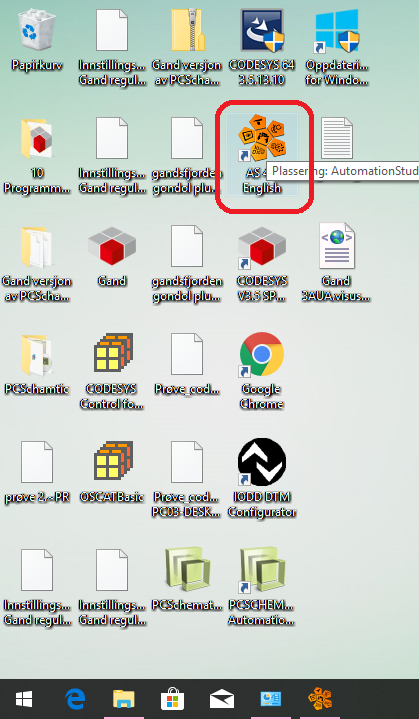
\includegraphics[width=0.5\textwidth]{stasjon07x09.png}
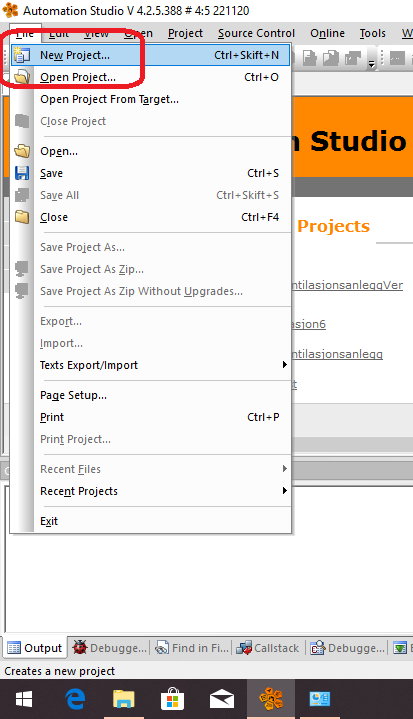
\includegraphics[width=0.5\textwidth]{stasjon07x01.png}

\newpage{}
\item Navngi det nye prosjektet med Uke ?? Elev Navn og trykk next

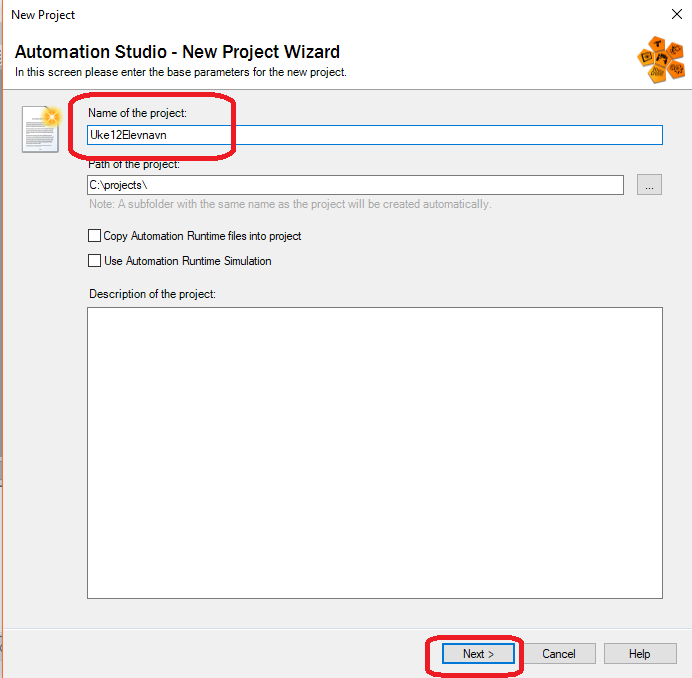
\includegraphics[width=0.5\textwidth]{stasjon07x02.png}
\item Velg Identify hardware configuration online

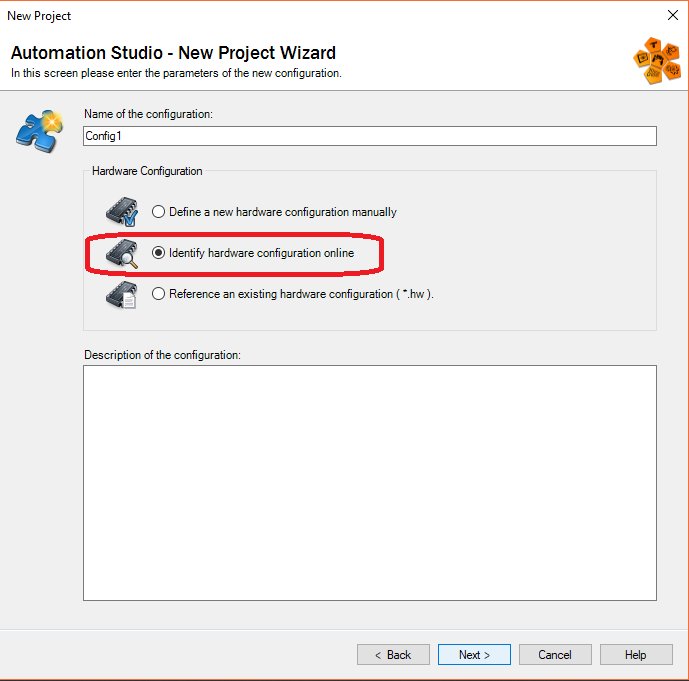
\includegraphics[width=0.5\textwidth]{stasjon07x03.png}
\newpage{}
\item Trykk identify Hardware og trykke finish når PLS-en er funnet. 

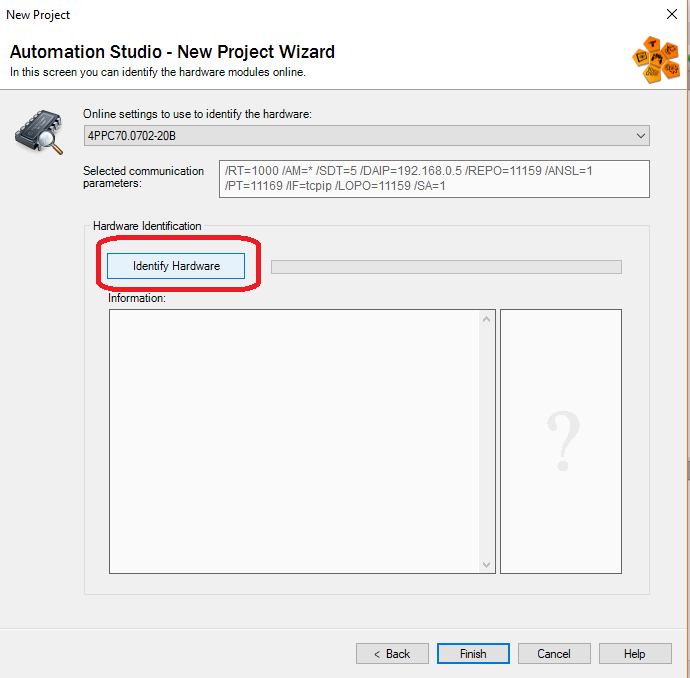
\includegraphics[width=0.5\textwidth]{stasjon07x04.png}
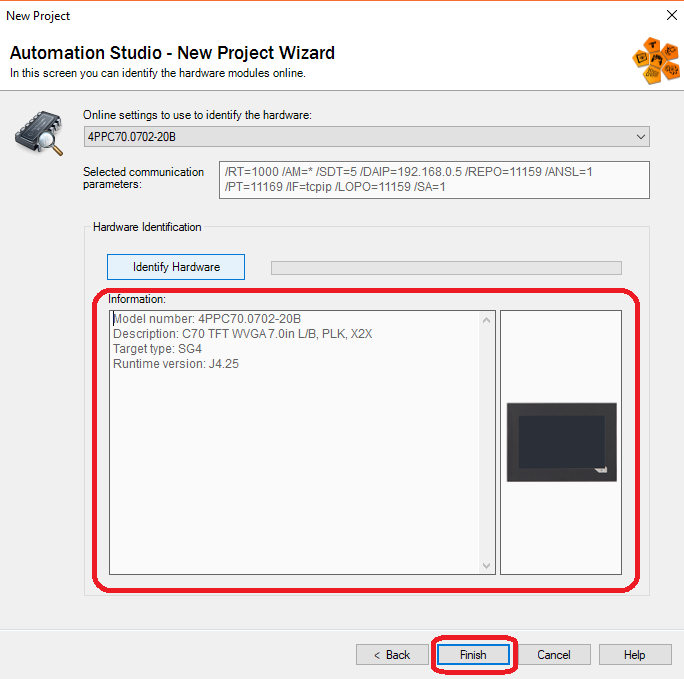
\includegraphics[width=0.5\textwidth]{stasjon07x05.png}
\item Nå skal du importere et standardprosjekt inn i det nye prosjektet. 

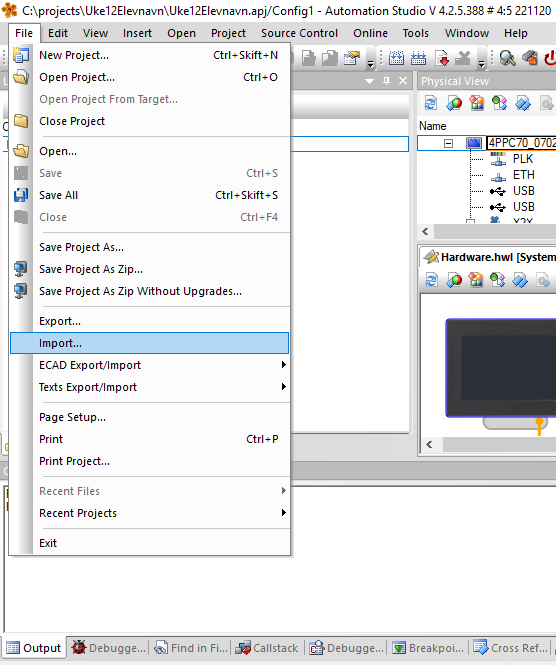
\includegraphics[width=0.5\textwidth]{stasjon07x06.png}
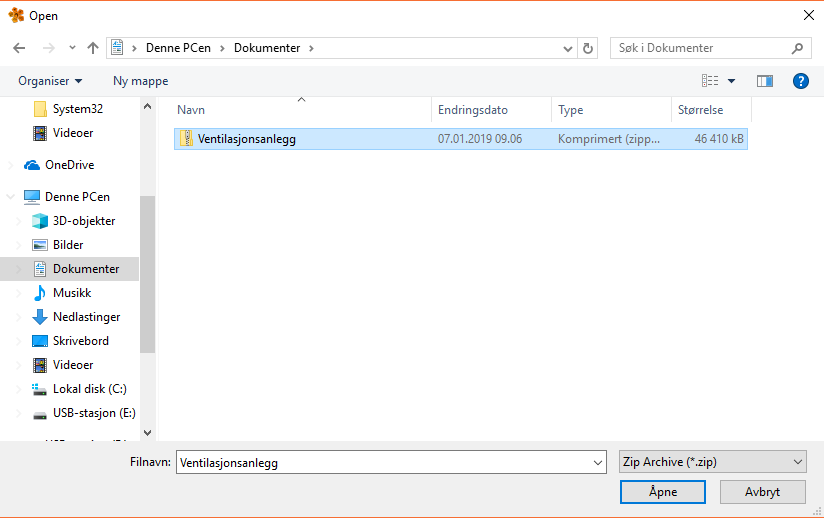
\includegraphics[width=0.5\textwidth]{stasjon07x07.png}\\
\newpage{}
\item Når prosjektet er lastet skal du gå inn på de fysiske inngangene.
Da må du velge Physical View. Du vil da få en oversikt over alt som
er koblet til PLS-en. RIO-en er tilkoblet med X2X buss, slik at om
du utvider denne vil du få en oversikt over alle IO-moduler. Gjør
deg kjent med disse ved å lese i manualen. 

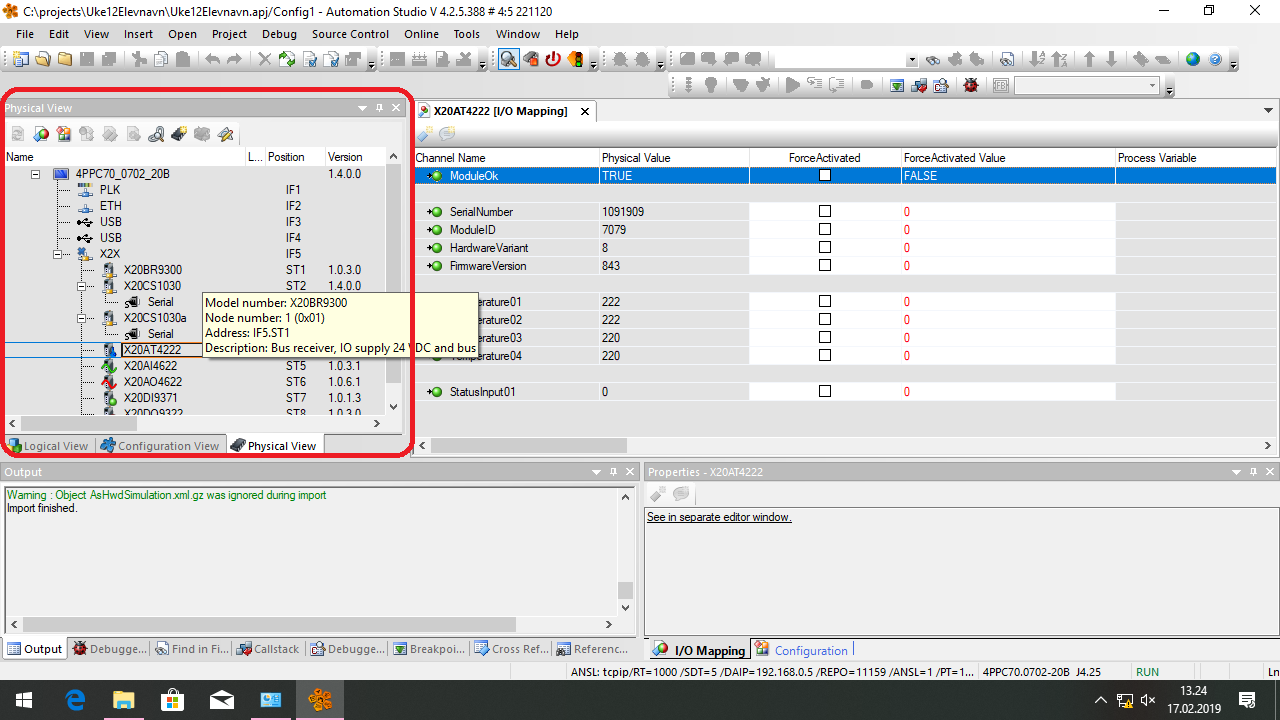
\includegraphics[width=1\textwidth]{stasjon07x08.png}
\end{enumerate}

Du skal gjøre en sjekk av alle inn- og utsignaler på anlegget (IO-sjekk)

Først må du identifisere alle signaler og sette opp en sjekkliste
(gjerne i execl, denne listen skal fremvises for godkjenning)

Koble deg til anlegget med tilhørende PC og utfør IO-sjekken. 

Sjekk: Lærer sjekker at IO-listen er utfylt og sjekker selv noen av
signalene. Lærer stiller også spørsmål til eleven om virkemåtene til
noen av sensorene på anlegget. 

\begin{center}
\begin{tabular}{ | m{8cm} | m{1cm}| m{2cm} | } 
\hline
\multicolumn{3}{|c|}{Punkter som skal godkjennes før en går videre på neste nivå} \\
	\hline
	Oppgave	& Utført & Signatur \\ 
	\hline
	\hline
Nytt prosjekt opprettet med rett navn	& & \\ 
	\hline
Har funnet feil oppsett med IO-moduler	& & \\ 
	\hline
Har dokumentert IO-sjekk	& & \\ 
	\hline
Eleven vet hvilket utstyr som er koblet til alle IO-er	& & \\ 
	\hline
Elven kan forklare virkemåten til et utvalg sensorer.	& & \\ 
	\hline
\end{tabular}
\end{center}
\newpage
\subsection*{Arbeidsoppdrag 2 - Fikse feil i PLC program}

Det er en feil i PLS programmet som gjøre at flowregulering ikke virker. 

Sjekk: lærer sjekker at regulering av strømning virker og ber eleven forklar hva som var problemet.
\newpage
\subsection*{Arbeidsoppdrag 3 - programmering av program for oppstart}

Du skal lage styreprogram for oppstart og stopp og ventilasjonsanlegg

Sekvens:
\begin{enumerate}
\item Init -- Ingen action |  start
\item Steg1 -- Spjeld åpnes | pause 30 sek
\item Steg2 -- Vifte startes med fast valgbar hastighet | Innstilt trykk over vifte
\item Steg3 --  Start hastighetsregulering | Stopp knapp
\item return to Init
\end{enumerate}

\subsection*{Arbeidsoppdrag 4 - Lage HMI bilde for styring}

Du skal lage et HMI bilde som viser en P \& ID av anlegget med tilhørende
styringsmuligheter
\underbar{file arb07.tex}

\end{document}

